\chapter{Desarrollo}
En este capítulo se presenta el método empleado para preprocesar los mamogramas
digitales.

\shorthandoff{>} % hack to combine tikZ and Spanish
    
% -------------------------------------------------
% Set up a new layer for the debugging marks, and make sure it is on
% top

\pgfdeclarelayer{marx}
\pgfsetlayers{main,marx}
% A macro for marking coordinates (specific to the coordinate naming
% scheme used here). Swap the following 2 definitions to deactivate
% marks.
\providecommand{\cmark}[2][]{%
  \begin{pgfonlayer}{marx}
    \node [nmark] at (c#2#1) {#2};
  \end{pgfonlayer}{marx}
  } 
\providecommand{\cmark}[2][]{\relax} 
% -------------------------------------------------
\begin{figure}[h]
\begin{center}
\begin{tikzpicture}[%
    >=triangle 60,              % Nice arrows; your taste may be different
    start chain=going below,    % General flow is top-to-bottom
    node distance=6mm and 60mm, % Global setup of box spacing
    every join/.style={norm},   % Default linetype for connecting boxes
    ]

{\small\ttfamily\fontfamily{lmodern}\selectfont
% ------------------------------------------------- 
% A few box styles 
% <on chain> *and* <on grid> reduce the need for manual relative
% positioning of nodes
\tikzset{
  base/.style={draw, on chain, on grid, align=center, minimum height=4ex},
  proc/.style={base, rectangle, text width=8em},
  test/.style={base, diamond, aspect=2, text width=5em},
  term/.style={proc, rounded corners},
  % coord node style is used for placing corners of connecting lines
  coord/.style={coordinate, on chain, on grid, node distance=6mm and 25mm},
  % nmark node style is used for coordinate debugging marks
  nmark/.style={draw, cyan, circle, font={\sffamily\bfseries}},
  % -------------------------------------------------
  % Connector line styles for different parts of the diagram
  norm/.style={->, draw, blue},
  free/.style={->, draw, green},
  cong/.style={->, draw, red},
  it/.style={font={\small\itshape}}
}
% -------------------------------------------------
% Start by placing the nodes
% Use join to connect a node to the previous one a

\node [term, it] (p0) {Start};
\node [proc, fill=violet!30, join] (p1) {Reduction of work area};
\node [test, join] (t1) {12 bits image?};
% No join for exits from test nodes - connections have more complex
% requirements
% We continue until all the blocks are positioned
\node [proc, fill=brown!30] (p2) {Conversion to 16 bits};
\node [proc, fill=blue!30, join] (p3) {Adaptive Median Filter};
\node [proc, fill=green!30, join] (p4) {Histogram Equalization};
\node [proc, fill=red!30, join] (p5) {Image shrinking};
\node [term, join, it]      {End};
% We position the next block explicitly as the first block in the
% second column.  The chain 'comes along with us'. The distance
% between columns has already been defined, so we don't need to
% specify it.

% -------------------------------------------------
% Now we place the coordinate nodes for the connectors with angles, or
% with annotations. We also mark them for debugging.

\node [coord, left=of t1]  (c1)  {}; %\cmark{1}   
 
% -------------------------------------------------
% A couple of boxes have annotations

% -------------------------------------------------
% All the other connections come out of tests and need annotating
% First, the straight north-south connections. In each case, we first
% draw a path with a (consistently positioned) annotation node, then
% we draw the arrow itself.
\path (t1.south) to node [near start, xshift=1em] {$yes$} (p2);
  \draw [->,blue] (t1.south) -- (p2);

% -------------------------------------------------
% Finally, the twisty connectors. Again, we place the annotation
% first, then draw the connector
\path (t1.west) to node [near start, yshift=-1em] {$no$} (c1); 
  \draw [->,blue] (t1.west) -- (c1) |- (p2);

% -------------------------------------------------

    \draw[brown, thick] ($(p3.north west)+(-0.3,0.3)$)  rectangle ($(p5.south east)+(0.3,-0.3)$) 
    node [right]{label};
}
\end{tikzpicture}
\end{center}
  \caption{Preprocessing method applied to each image in the collection} 
  \label{fig:flowchart} 
\end{figure}

\shorthandon{>} 

\section{Etapa de recolección}
Las mamografías originalmente almacenadas en discos compactos, fueron extraídas
y ... , removimos los datos privados de las imágenes, los únicos campos son los
que se muestran en la \ref{table:dicomtags} 

\begin{table}[h]
  \caption{Etiquetas DICOM que permanecen en la imagen} 
  \label{table:dicomtags}
\begin{center}
{\small
    \begin{tabular}{c|c}
    \hline

    {\bf Etiquetas} & 
    {\bf Descripción} \\
    \hline
           (0000, 0001) & Bits alojados \\
           (0000, 0001) & Bits alojados \\
           (0000, 0001) & Bits alojados \\
           (0000, 0001) & Bits alojados \\
    \hline
    \end{tabular}
}
\end{center}
\end{table}

%Las tareas de \textit{scripting} se llevaron a cabo con el lenguaje de
%programación Python y la libreria PyDICOM.

\section{Método}
Se eligió un método híbrido

\subsection{Reducción del área de trabajo}

La primera etapa del método consiste en eliminar la región oscura que cubre
gran parte de la imagen para acelerar el tiempo de ejecución de los
procedimientos posteriores. El enfoque es similar al expuesto por Dehghani y
Holguín \cite{dehghani2011method, holguinpre}.

\subsection{Conversión de bits}

Las mamografías que se obtuvieron son de 12 bits. Sin embargo al visualizarlas
se obtiene una imagen opaca, esto es porque ...

\subsection{Eliminación de ruido}
Se elimina el ruido.

\subsection{Mejora del contraste}
Se mejora el contraste.

\subsection{Compresión} \label{compression}

%This is the final phase in our method. It deals with image compression. A
%compressed image takes less time for transmission, processing, and less storage
%capacity. We applied a technique introduced by AbuBaker
%\cite{abubaker2006mammogram}  abubaker2007efficient}. It aims at compressing an
%image with minimal loss of quality. 
%
%%We introduced small changes to the original method, making the bit conversion
%%with the algorithm proposed for the enhancement and applying after that a
%%normalization step.
%
%The applied method consists of three steps: image shrinking procedure, pixel
%depth conversion, and image enhancement. Description of each step follows. 
%
%\subsubsection{Image shrinking procedure.} 
%Here, we will find the maximum shrinking level of the image. It takes three
%substeps:
%
%\begin{enumerate}[a)]
%    \item Obtain the image histogram (see Fig. \ref{comp:a} and \ref{comp:b}). %% DESCRIBIR QUE SE HIZO AQUI
%    \item Modify the histogram by deleting the unused gray levels (gaps) in the
%    histogram. The result will be a right-skewed histogram, as shown in Fig.
%    \ref{comp:c}.  
%    \item Generate an image based on the new histogram. The new image will be
%    quite dark due to the gray levels being located in the dark side section, Fig. \ref{comp:d}.
%\end{enumerate}
%
%\begin{figure}[h]
%  \begin{center}
%    \hspace{\fill}
%    \subfloat[\label{comp:a}]{\includegraphics[height=30mm]{images/original-mammogram-16bits}}
%    \hfill
%    \subfloat[\label{comp:b}]{\includegraphics[height=30mm]{images/original-image-histogram}}
%    \hfill
%    \subfloat[\label{comp:c}]{\includegraphics[height=30mm]{images/shrunk-histogram}}
%    \hfill
%    \subfloat[\label{comp:d}]{\includegraphics[height=30mm]{images/dark-mammogram}}
%    \hspace{\fill}
%  \end{center}
%
%  \caption{Shrinking procedure. \subref{comp:a} original mammogram,
%  \subref{comp:b} histogram of \subref{comp:a}, \subref{comp:c} histogram shown
%  in \subref{comp:b} after being shrunk, and \subref{comp:d} is the dark image
%  generated from the shrunk histogram.} 
%  
%  \label{img:shrinking-one} \end{figure}
%
%%\begin{verbatim}
%
%%\end{verbatim}
%
%\subsubsection{Pixel depth conversion.} 
%In this step the goal is to reduce the size of the image. Three substeps are
%involved:
%
%\begin{enumerate}[a)] %% NECESITAMOS AGREGAR DESCRIPCION DE CADA UNO DE ESTOS SUBSTEPS
%    \item Extract the histogram of the shrunk image.
%    \item Find the maximum shrinking level for the image.
%    \item Reduce image from 16 to 8 bits. 
%\end{enumerate}
%
%The shape of the original histogram shown in Fig. \ref{comp:b} is quite similar
%to the histogram of the resultant image shown in Fig. \ref{comp:g}. Peaks look
%the same, which indicates that the concentration of gray levels remains
%unchanged.
%
%\begin{figure}[h]
%  \begin{center}
%    \hspace{\fill}
%    \subfloat[\label{comp:e}]{\includegraphics[height=30mm]{images/dark-mammogram-histogram}}
%    \hfill
%    \subfloat[\label{comp:f}]{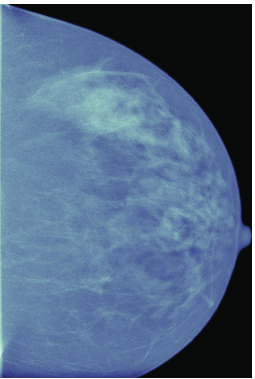
\includegraphics[height=30mm]{images/compressed-mammogram-8bits}}
%    \hfill
%    \subfloat[\label{comp:g}]{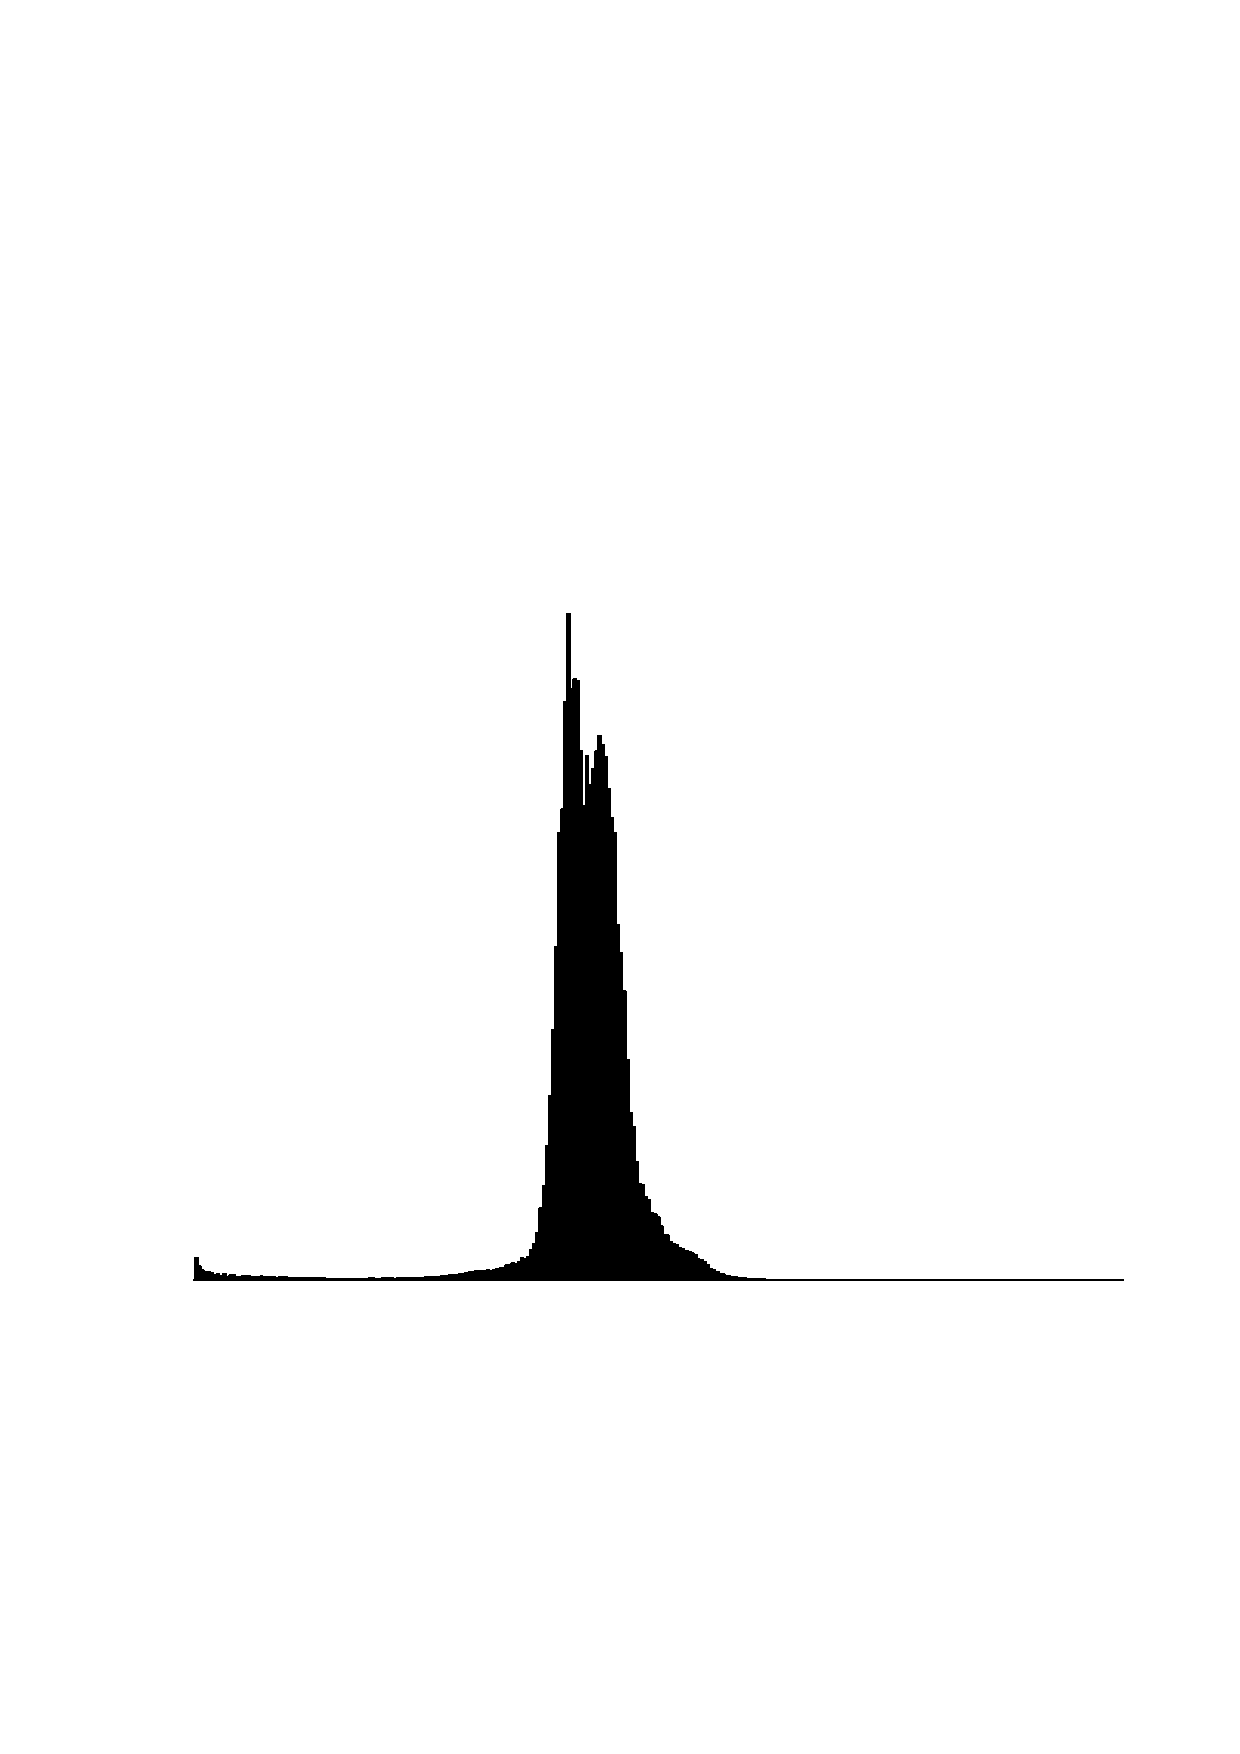
\includegraphics[height=30mm]{images/compressed-mammogram-histogram}}
%    \hspace{\fill}
%  \end{center}
%
%  \caption{(a) shows histogram generated from the dark mammogram, (b) is the 8 
%  bits mammogram, and (c) is the histogram of 8-bit image, which is similar to 
%  the original mammogram.} 
%  
%  \label{img:shrinking-two}
%\end{figure}
%
%\subsubsection{Enhancing pixel depth conversion.}
%This step aims at improving brightness of the image obtained from pixel depth
%conversion.  Afterwards, image conversion from 16 to 8 bits using an efficient
%coefficient takes place.  Medical information carried by the image should be
%maintained. %% AGREGAR REFERENCIA A UNA FIG., SI LA HAY

% change the words in this paragrap

%This final step is useful like a normalization process. Below is presented the 
%Matlab code used:

\definecolor{bg}{rgb}{0.9,0.9,0.9}
\begin{minted}[linenos=true, 
               %fontfamily=fi4, 
               fontseries=ubx,
               bgcolor=bg, frame=lines]{matlab}
% Get the size of the image
% Based on Abubaker code
[height width] = size(image);
imageCopy = repmat(uint8(0), height, width);
divider = 0.0;
maxLevel = double(usedGrayLevels);

while 1
    divider = divider + 0.01;
    if maxLevel/divider <= 255
        break;
    end
end
fprintf('text');
for h=1:1:height
    for w=1:1:width
       imageCopy(h, w) = image(h, w)/divider;
    end
end
\end{minted}

%Recordar escribir que en las primeras pruebas sólo se mejoró  la visualización
%del tejido graso y no del tejido mamario.


